\capituloUDA{Análisis comparativo y propuesta de optimización}{Del diagnóstico a la propuesta verificable}{%
  \itemCapituloUDA{-2.15}{Brechas del caso base y prioridades}
  \itemCapituloUDA{-3.18}{Definición de los paquetes de mejora}
  \itemCapituloUDA{-4.21}{Resultados y comparación de escenarios}
  \itemCapituloUDA{-5.24}{Respuesta a la matriz de sostenibilidad}
  \itemCapituloUDA{-6.27}{Implementación y lineamientos replicables}
  \itemCapituloUDA{-7.30}{Síntesis y alcance de la validación}
}
\begin{textoDosTercios}
Este capítulo desarrolla la propuesta de optimización a partir de la matriz del capítulo 3 y del diagnóstico del capítulo 4. La secuencia relaciona cada brecha con una intervención, sus parámetros de simulación y la evidencia necesaria para evaluar su desempeño. Las comparaciones energéticas se distinguen de los requisitos de confort, agua, materiales y gestión que requieren comprobaciones adicionales.

Se conservan los ensayos C1, C2 y C3 revisión 01 como registro de la primera comparación. C3 revisión 02 amplía el paquete combinado para responder a las brechas detectadas. Esta evolución no modifica retrospectivamente las entradas ni los resultados de los ensayos anteriores.
\end{textoDosTercios}

\section{Brechas del caso base y prioridades de intervención}
\begin{textoDosTercios}
La aplicación de la matriz identifica una potencia de iluminación de 10, 15 y 25 W/m\textsuperscript{2} en las 19 zonas con iluminación artificial. Estos valores superan el umbral de 8 W/m\textsuperscript{2} adoptado en E05. La primera prioridad consiste en reducir esta carga sin reducir arbitrariamente la iluminancia requerida para las actividades.

La envolvente constituye la segunda prioridad: el ensayo reflectante actúa sobre la absorción solar, pero no incorpora aislamiento adicional ni mejora el vidrio. La ventilación natural y las protecciones exteriores requieren evaluar conjuntamente energía, luz natural y confort. Las aberturas propuestas no demuestran por sí mismas renovación de aire suficiente.

La tercera prioridad reúne la evidencia ajena al balance térmico: consumo de agua, carbono incorporado, emisiones de productos, eficiencia de equipos, generación renovable y mantenimiento. Cada componente recibe una acción y un documento de cierre en la sección de implementación, evitando inferir cumplimiento ambiental a partir de una sola reducción energética.
\end{textoDosTercios}

\section{Definición de los paquetes de optimización}
\begin{textoDosTercios}
C1 permite estudiar un paquete pasivo localizado; C2 aísla el efecto óptico de un acabado de cubierta; C3 revisión 01 combina ambos. C3 revisión 02 corresponde a una propuesta ampliada de envolvente e iluminación. Por tanto, la revisión 02 se compara directamente con el CB y con su antecedente, pero no se interpreta como la suma de los efectos de C1 y C2.
\end{textoDosTercios}
% Estrategias propuestas: no son resultados de simulación.
\clearpage
\subsection{Escenario pasivo (C1)}
\label{sec:c1-propuesta}

El escenario C1 se plantea como un paquete organizado en cinco criterios: protección solar exterior, área libre de ventanas, recorrido del aire por el atrio, control de la ventilación natural y aprovechamiento de luz natural. Se ha preparado una copia independiente del modelo base; las medidas descritas a continuación todavía no se han aplicado ni simulado. Por tanto, este apartado define la propuesta de ensayo y no demuestra ahorros energéticos.

Para aislar el efecto de C1, se conservarán la orientación, la materialidad, el clima, la ocupación, las cargas y las consignas del caso base. Los cambios en capas o propiedades térmicas de la envolvente se reservan para C2. La cubierta del atrio y las rejillas superiores forman parte de la configuración base y se mantienen.

\subsubsection{Criterio 1: protección solar exterior}
La primera estrategia consiste en complementar las protecciones donde su cobertura resulte insuficiente. El modelo ya contiene celosías y voladizos, por lo que se debe comprobar su geometría antes de añadir aleros o lamas. La figura~\ref{fig:c1-solar} expresa el criterio de intervención; sus dimensiones se definirán por ventana y orientación. La evaluación conjunta de energía e iluminación permitirá reconocer posibles penalizaciones de luz natural.

\begin{figure}[H]
\centering
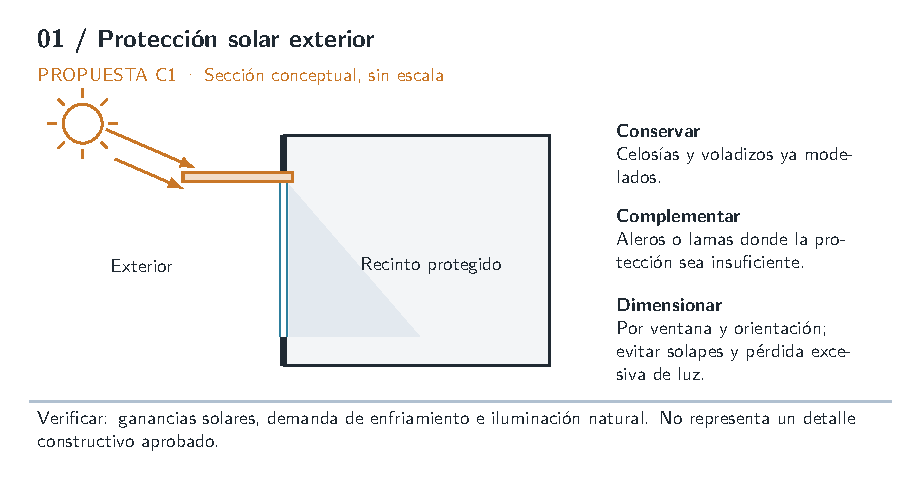
\includegraphics[width=\textwidth]{figuras/c1/c1-proteccion-solar.pdf}
\caption{Criterio propuesto de protección solar exterior para C1.}
\label{fig:c1-solar}
\fuente{Elaboración propia a partir de la revisión del modelo base en DesignBuilder. Esquema conceptual sin escala; geometría adicional pendiente de dimensionamiento.}
\end{figure}

\clearpage
\subsubsection{Criterio 2: área libre de ventanas}
Se propone evaluar una fracción practicable del 20\,\% en ventanas exteriores de oficinas. El valor del 5\,\% se observó en el nivel general del edificio y en la zona 1PA-OF-02; no se extiende automáticamente a todas las ventanas. El 20\,\% constituye un parámetro propuesto de ensayo, pendiente de comprobar mediante el tipo de hoja, el área libre efectiva y su compatibilidad con las celosías.

La figura~\ref{fig:c1-aperturas} distingue el valor observado del parámetro propuesto. La selección de ventanas deberá considerar su operación real, accesibilidad y compatibilidad con las protecciones exteriores.

\begin{figure}[H]
\centering
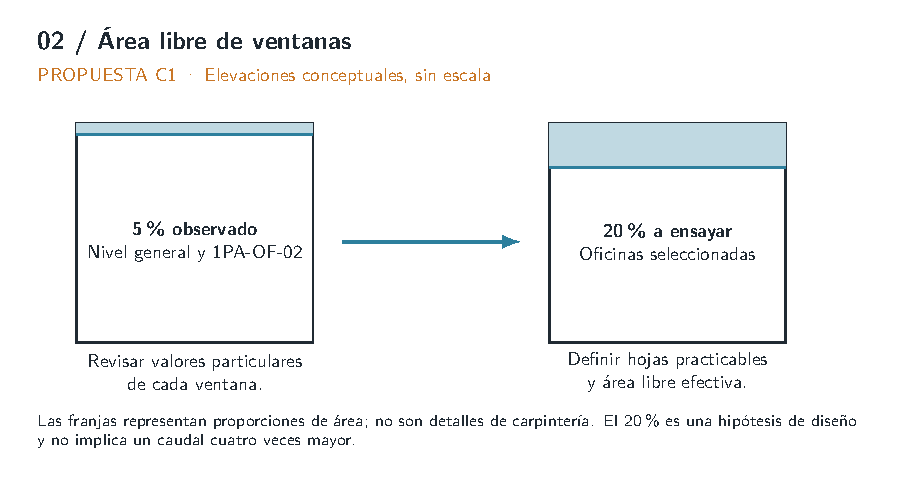
\includegraphics[width=\textwidth]{figuras/c1/c1-aperturas.pdf}
\caption{Fracción de apertura observada y propuesta de ensayo en ventanas de oficinas.}
\label{fig:c1-aperturas}
\fuente{Elaboración propia. Proporciones conceptuales; no representan dimensiones de hojas ni resultados de ventilación.}
\end{figure}

\clearpage
\subsubsection{Criterio 3: recorrido del aire por el atrio}
La figura~\ref{fig:c1-aire} representa el recorrido que se debe verificar entre exterior, oficinas, pasillos y atrio. El atrio comienza en la primera planta alta y conserva su cubierta. Las flechas no representan resultados de caudal ni prueban ventilación cruzada: se comprobarán las conexiones interiores efectivas y la respuesta de la red de flujo de aire. No se presuponen nuevos pasos en divisiones cerradas.

\begin{figure}[H]
\centering
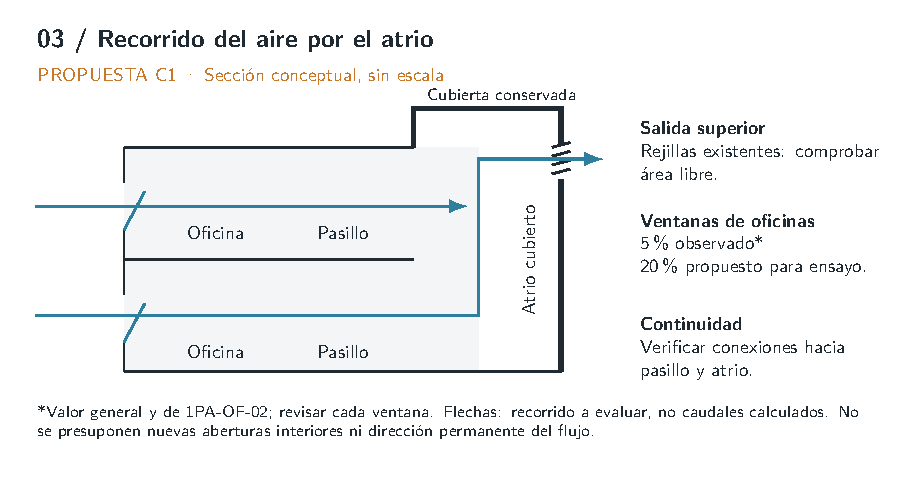
\includegraphics[width=\textwidth]{figuras/c1/c1-ventilacion-atrio.pdf}
\caption{Esquema del recorrido de aire a evaluar y propuesta de apertura de ventanas para C1.}
\label{fig:c1-aire}
\fuente{Elaboración propia. Sección conceptual, sin escala, basada en el atrio cubierto del modelo. Las conexiones, áreas libres y caudales requieren verificación.}
\end{figure}

\clearpage
\subsubsection{Criterio 4: control de la ventilación natural}
El cuarto criterio plantea coordinar la apertura de ventanas con el horario de uso y la demanda de refrigeración. La secuencia de la figura~\ref{fig:c1-control} requiere definir y comprobar los umbrales interiores y exteriores, las restricciones de operación y el comportamiento del sistema cuando se habilita la ventilación natural. Se mantendrán las consignas del caso base para distinguir el efecto de la estrategia.

\begin{figure}[H]
\centering
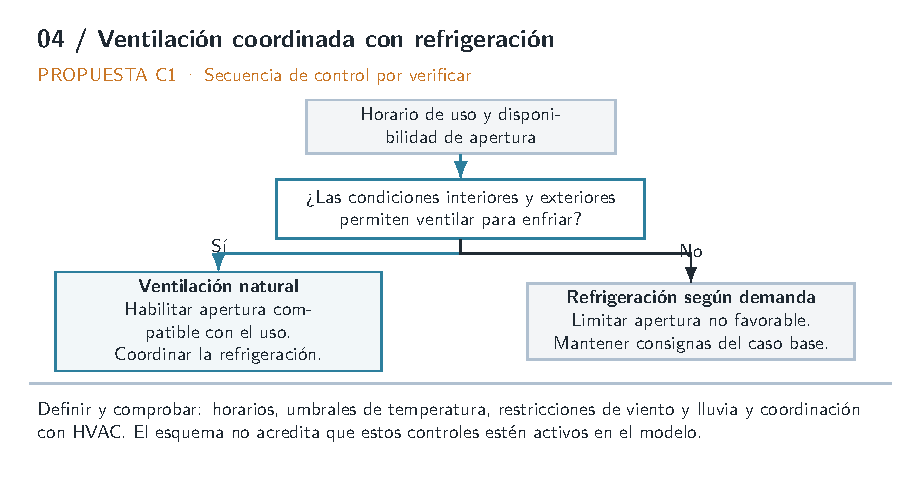
\includegraphics[width=\textwidth]{figuras/c1/c1-control-ventilacion.pdf}
\caption{Secuencia propuesta de coordinación entre ventilación natural y refrigeración para C1.}
\label{fig:c1-control}
\fuente{Elaboración propia. Lógica conceptual pendiente de configuración y verificación en el archivo de simulación; no representa controles ya implementados.}
\end{figure}

La evaluación considerará demanda térmica sensible y total, electricidad estimada de refrigeración, temperaturas durante horas ocupadas y ventilación por zona. La iluminación natural se recalculará con las mismas condiciones del caso base. Los resultados heredados al copiar el archivo no se utilizarán como resultados de C1.

\clearpage
\subsubsection{Criterio 5: aprovechamiento de luz natural}
El quinto criterio consiste en ajustar la geometría de las protecciones para equilibrar el control solar y la entrada de luz natural, como se representa en la figura~\ref{fig:c1-luz}. Se evaluarán profundidad y separación de aleros o lamas, manteniendo el vidrio y las reflectancias del caso base. Este criterio complementa la protección solar y no constituye una sustitución de materiales.

La comparación se realizará con cielo CIE cubierto de 10000 lux, plano de trabajo a 0,76 m y malla de 0,30 m. Se revisarán la distribución de iluminancia y la proporción de área que supera FLD 2\,\%. Este ensayo estático no permite afirmar autonomía lumínica anual ni ausencia de deslumbramiento. Tampoco se atribuirá ahorro de electricidad de iluminación sin modelar y evaluar el control correspondiente.

\begin{figure}[H]
\centering
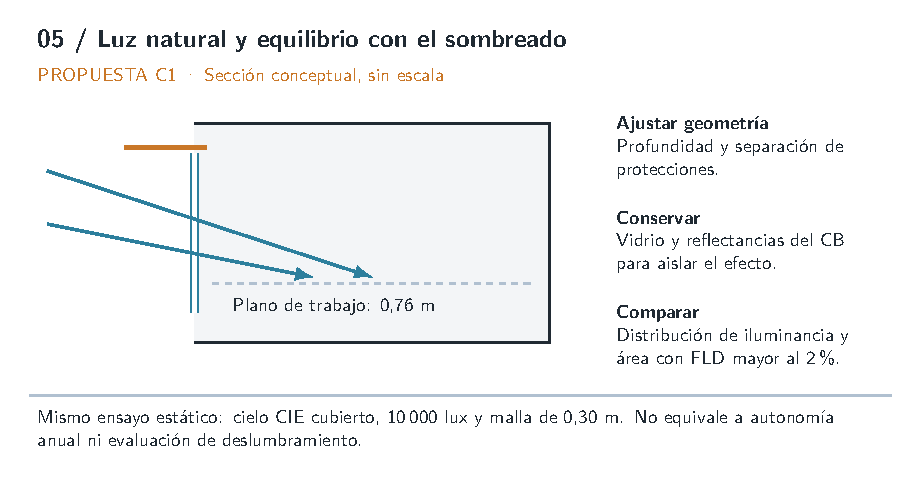
\includegraphics[width=\textwidth]{figuras/c1/c1-iluminacion-natural.pdf}
\caption{Criterio de equilibrio entre protección solar y aprovechamiento de luz natural.}
\label{fig:c1-luz}
\fuente{Elaboración propia. Sección conceptual; condiciones de cálculo equivalentes al ensayo estático del caso base.}
\end{figure}

Los cinco criterios se evaluarán como un paquete C1. El área libre, el recorrido del aire y su control son aspectos complementarios de la ventilación; una sola corrida conjunta no permite atribuir por separado los ahorros a cada criterio. Para ello serían necesarios ensayos adicionales modificando una variable cada vez.

\clearpage
\subsubsection{Registro de intervención y validación}
La tabla~\ref{tab:c1-paquete} distingue las condiciones observadas de las decisiones propuestas. Antes de la comparación final se deberán resolver o justificar las incidencias del caso base relativas al datacenter, al dimensionamiento de invierno y a la geometría de la red de aire. Cualquier corrección de una entrada común exigirá actualizar también la simulación base.

\begin{table}[H]
\centering
\caption{Parámetros y verificaciones del paquete pasivo C1.}
\label{tab:c1-paquete}
{\fontsize{9}{11}\selectfont
\begin{tabular}{p{2.4cm}p{3.1cm}p{3.1cm}p{3.1cm}}
\toprule
Medida & Condición base & Propuesta C1 & Verificación pendiente \\
\midrule
Protección solar & Celosías y voladizos modelados. & Complementar protección insuficiente. & Dimensiones, orientación, solapes y luz natural. \\
\addlinespace
Ventanas & Apertura de 5\,\% observada a nivel general y en 1PA-OF-02. & Ensayar 20\,\% en ventanas de oficinas seleccionadas. & Inventario por ventana, tipo de hoja y área libre. \\
\addlinespace
Atrio & Cubierta, pasos abiertos y rejillas superiores. & Conservar y verificar el recorrido del aire. & Conectividad, aberturas horizontales y caudales. \\
\addlinespace
Operación & Controles particulares del modelo base. & Coordinar ventanas y refrigeración. & Horarios, umbrales y control exportado. \\
\addlinespace
Luz natural & Ensayo estático actualizado del CB. & Ajustar protecciones conservando vidrio y reflectancias. & Iluminancia y área con FLD mayor al 2\,\%. \\
\bottomrule
\end{tabular}}
\fuente{Elaboración propia a partir de la revisión del modelo y de la propuesta de ensayo. Ninguna fila acredita una medida simulada.}
\end{table}

La validación seguirá la secuencia: definir el paquete, aplicar los cambios en la copia C1, contrastar el archivo exportado con CB, ejecutar las simulaciones y comparar los indicadores. La combinación de medidas pasivas con sustituciones de materiales corresponderá a C3, después de evaluar C1 y C2 por separado.

\clearpage

\clearpage
\subsection{Escenario material C2 y combinación inicial C3}
C2 revisión 01 cambia la absortancia solar del acabado de cubierta de 0,40 a 0,20. C3 revisión 01 conserva esa hipótesis y las medidas pasivas de C1. La modificación es una sensibilidad óptica; la denominación del escenario material no acredita que el producto sea de bajo carbono, reciclado o de bajas emisiones.
\clearpage
\subsection{Propuesta ampliada C3 revisión 02}
\label{sec:c3-revision02}
La revisión 02 conserva el paquete pasivo y el acabado reflectante e incorpora tres grupos de ajustes: aislamiento de elementos opacos, vidrio de control solar y reducción de potencia de iluminación con regulación por luz natural. Los valores son especificaciones de desempeño del ensayo; la selección comercial permanece condicionada a fichas técnicas y verificación constructiva.
\begin{table}[H]\centering
\caption{Parámetros propuestos para C3 revisión 02}
{\small\singlespacing\renewcommand{\arraystretch}{1.25}
\begin{tabular}{>{\raggedright\arraybackslash}p{2.4cm}>{\raggedright\arraybackslash}p{6.2cm}>{\raggedright\arraybackslash}p{4.7cm}}\toprule
Componente & Ajuste del ensayo & Condición de verificación \\ \midrule
Cubierta & 80 mm de aislante de $\lambda=0,040$ W/(m K); acabado reflectante conservado. $U$ nominal de capas: 0,267 W/(m\textsuperscript{2} K). & Continuidad, humedad, puentes térmicos y propiedades del producto. \\
Muro exterior & 60 mm del mismo aislante; $U$ nominal de capas: 0,534 W/(m\textsuperscript{2} K). & Compatibilidad del revestimiento y fijación; no modifica divisiones interiores. \\
Vidrio exterior & $U=1,8$ W/(m\textsuperscript{2} K), SHGC 0,35 y transmisión visible 0,65. Marcos conservados. & Parámetros del centro del vidrio; verificar conjunto y sombreado eficaz. \\
Iluminación & 8 W/m\textsuperscript{2} en 19 zonas; regulación continua por luz natural. & Fotometría LED, ubicación de sensores y respuesta horaria del control. \\
Cotejo & Clima, geometría, horarios, ocupación, equipos y consignas conservados. & Nueva corrida anual y cotejo de entradas exportadas. \\
\bottomrule\end{tabular}}
\fuente{Elaboración propia. Especificaciones hipotéticas; transmitancias unidimensionales calculadas con capas y resistencias superficiales del modelo. No incluyen puentes térmicos.}
\end{table}
Los cambios de iluminación son una medida complementaria de eficiencia operacional, distinta de las estrategias pasivas. La menor potencia no se obtiene reduciendo la iluminancia objetivo. Se configuraron 19 controles, de los cuales seis no actúan por ausencia de ventanas exteriores. La regulación se evalúa con los puntos de referencia del modelo; su eficacia no sustituye un estudio anual de autonomía de luz natural y deslumbramiento.


\section{Resultados y comparación de escenarios}
\begin{textoDosTercios}
La comparación parte de corridas anuales independientes, con idéntico archivo climático y periodo de 8.760 horas. Se presenta primero la respuesta detallada de C1 y después el balance conjunto de la revisión 01. Los resultados de la revisión ampliada se identifican por separado para evitar mezclar versiones.
\end{textoDosTercios}
% Resultados propios C1 revisión 01; exportación auditada de EnergyPlus.
\clearpage
\subsection{Resultados preliminares del escenario pasivo C1}
\label{sec:c1-resultados}
La simulación anual de C1 reduce la demanda total de enfriamiento de 84.759,41 a 83.103,76 kWh térmicos, una diferencia de 1.655,65 kWh y una reducción del 1,95\,\% respecto al caso base. Esta magnitud incluye enfriamiento sensible y latente; no representa consumo eléctrico. La tabla~\ref{tab:c1-anual} conserva las 25 zonas con resultados de enfriamiento, incluidas aquellas con demanda nula.

\begin{table}[H]
\centering
\caption{Demanda anual de enfriamiento total por zona: caso base y C1.}
\label{tab:c1-anual}
{\fontsize{9}{11}\selectfont
\begin{tabular}{lrrrr}
\toprule
Zona & CB (kWh) & C1 (kWh) & C1 $-$ CB (kWh) & Variación \\
\midrule
PB-ASC & 0,00 & 0,00 & 0,00 & --- \\
PB-BA-01 & 0,00 & 0,00 & 0,00 & --- \\
PB-BO-01 & 0,00 & 0,00 & 0,00 & --- \\
PB-ES-01 & 0,00 & 0,00 & 0,00 & --- \\
PB-OF-01 & 2.800,60 & 2.639,71 & \textcolor[HTML]{2A9D8F}{-160,89} & \textcolor[HTML]{2A9D8F}{-5,74\,\%} \\
PB-OF-02 & 2.371,54 & 2.273,69 & \textcolor[HTML]{2A9D8F}{-97,85} & \textcolor[HTML]{2A9D8F}{-4,13\,\%} \\
PB-OF-03 & 3.062,20 & 2.984,56 & \textcolor[HTML]{2A9D8F}{-77,64} & \textcolor[HTML]{2A9D8F}{-2,54\,\%} \\
PB-RE-01 & 0,00 & 0,00 & 0,00 & --- \\
PB-SE-01 & 11.810,79 & 11.730,71 & \textcolor[HTML]{2A9D8F}{-80,08} & \textcolor[HTML]{2A9D8F}{-0,68\,\%} \\
1PA-BA-01 & 0,00 & 0,00 & 0,00 & --- \\
1PA-BA-02 & 0,00 & 0,00 & 0,00 & --- \\
1PA-DC & 40.196,11 & 40.147,08 & \textcolor[HTML]{2A9D8F}{-49,03} & \textcolor[HTML]{2A9D8F}{-0,12\,\%} \\
1PA-ES & 0,00 & 0,00 & 0,00 & --- \\
1PA-OF-01 & 4.447,65 & 3.948,92 & \textcolor[HTML]{2A9D8F}{-498,73} & \textcolor[HTML]{2A9D8F}{-11,21\,\%} \\
1PA-OF-02 & 2.967,62 & 2.837,18 & \textcolor[HTML]{2A9D8F}{-130,43} & \textcolor[HTML]{2A9D8F}{-4,40\,\%} \\
1PA-OF-03 & 4.500,53 & 4.059,70 & \textcolor[HTML]{2A9D8F}{-440,83} & \textcolor[HTML]{2A9D8F}{-9,80\,\%} \\
1PA-PAS & 0,00 & 0,00 & 0,00 & --- \\
1PA-SR & 3.053,31 & 3.014,99 & \textcolor[HTML]{2A9D8F}{-38,32} & \textcolor[HTML]{2A9D8F}{-1,25\,\%} \\
1PA-ASC & 0,00 & 0,00 & 0,00 & --- \\
2PA-BA-01 & 0,00 & 0,00 & 0,00 & --- \\
2PA-CAF & 2.642,02 & 2.638,45 & \textcolor[HTML]{2A9D8F}{-3,57} & \textcolor[HTML]{2A9D8F}{-0,14\,\%} \\
2PA-ES & 0,00 & 0,00 & 0,00 & --- \\
2PA-PAS & 0,00 & 0,00 & 0,00 & --- \\
2PA-SUM & 6.907,04 & 6.828,77 & \textcolor[HTML]{2A9D8F}{-78,27} & \textcolor[HTML]{2A9D8F}{-1,13\,\%} \\
2PA-ASC & 0,00 & 0,00 & 0,00 & --- \\
\midrule
\textbf{Total} & \textbf{84.759,41} & \textbf{83.103,76} & \textbf{$-$1.655,65} & \textbf{$-$1,95\,\%} \\
\bottomrule
\end{tabular}}
\fuente{Elaboración propia con resultados horarios de EnergyPlus, CB revisión 09 y C1 revisión 01, año de simulación 2025. Unidades térmicas. El guion indica una variación porcentual indefinida porque CB es cero.}
\end{table}

\clearpage
\subsubsection{Variación mensual por zona}
La figura~\ref{fig:c1-matriz-resultados} muestra que la respuesta del paquete varía durante el año. Algunas oficinas presentan aumentos de demanda entre enero y mayo, mientras que las reducciones son más pronunciadas en los meses posteriores. Los porcentajes comparan cada zona y mes con su propio valor base; no deben promediarse para obtener el ahorro anual del edificio.
\begin{figure}[H]
\centering
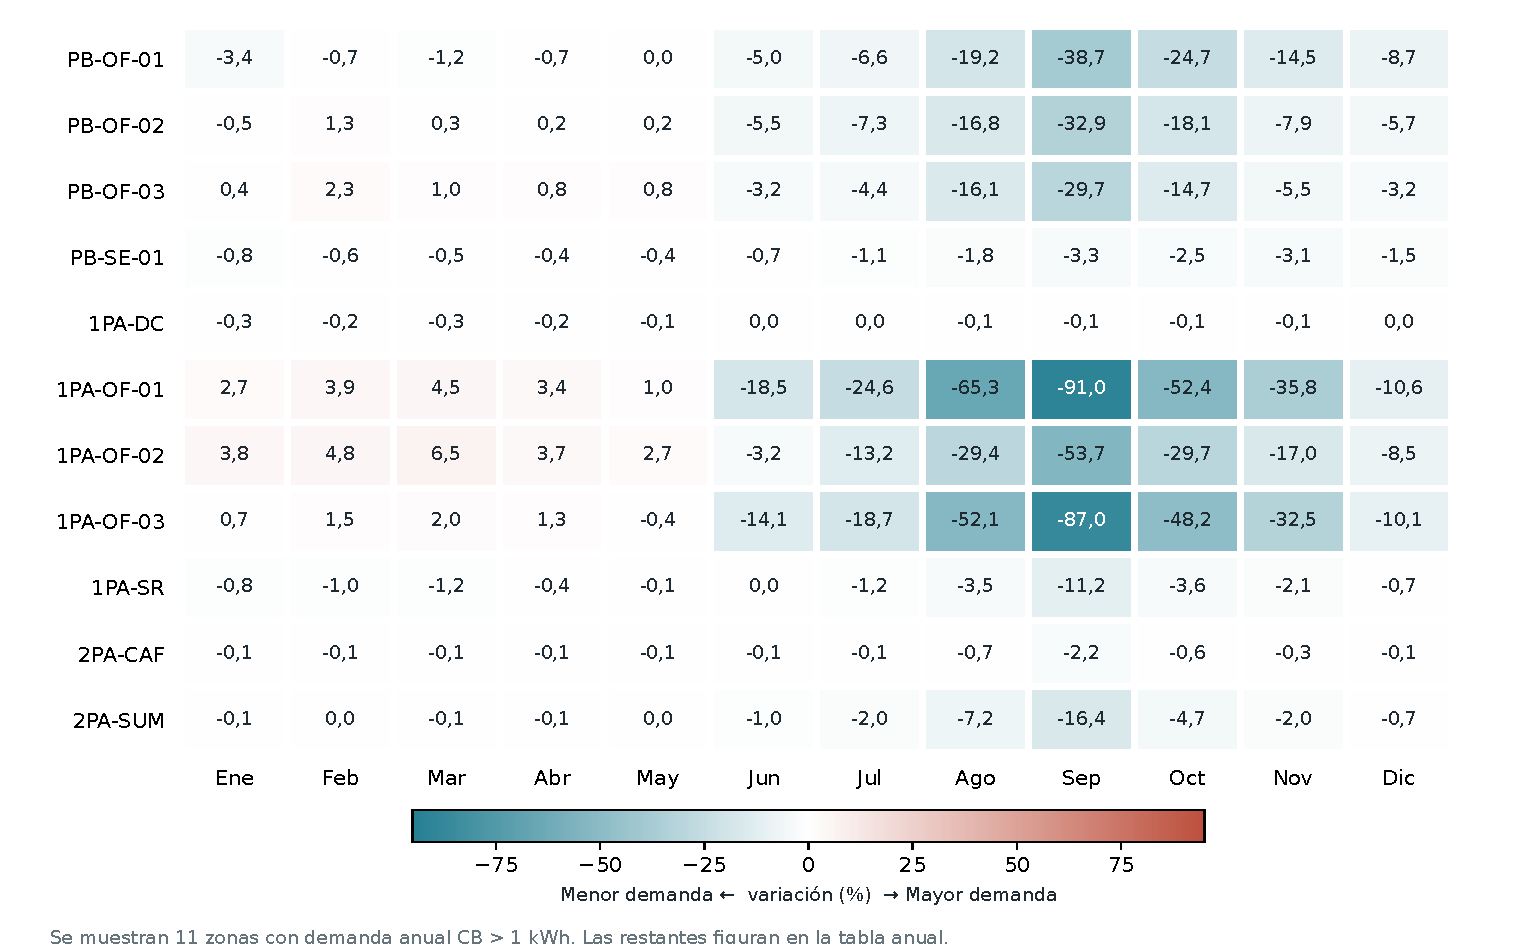
\includegraphics[width=\textwidth]{figuras/c1/02-matriz-mensual.pdf}
\caption{Variación porcentual mensual de la demanda de enfriamiento de C1 respecto al caso base.}
\label{fig:c1-matriz-resultados}
\fuente{Elaboración propia con resultados de EnergyPlus. Se muestran las 11 zonas con demanda anual base superior a 1 kWh. Turquesa: reducción; naranja: incremento. Variación = 100 $\times$ (C1 $-$ CB) / CB.}
\end{figure}

La reducción anual es preliminar. La corrida concluyó con 318 advertencias y ningún error severo, el mismo total de advertencias del CB. Esto acredita la finalización del cálculo, pero no resuelve los pendientes de entradas físicas, red de aire, confort ocupado e iluminación.

\clearpage
\subsubsection{Respuesta de las oficinas intervenidas}
Las seis oficinas presentan menor demanda anual en C1 (figura~\ref{fig:c1-oficinas-resultados}). La reducción oscila entre el 2,54\,\% en PB-OF-03 y el 11,21\,\% en 1PA-OF-01. Las conexiones representan pares de resultados de una misma oficina y no trayectorias temporales ni flujos de aire.
\begin{figure}[H]
\centering
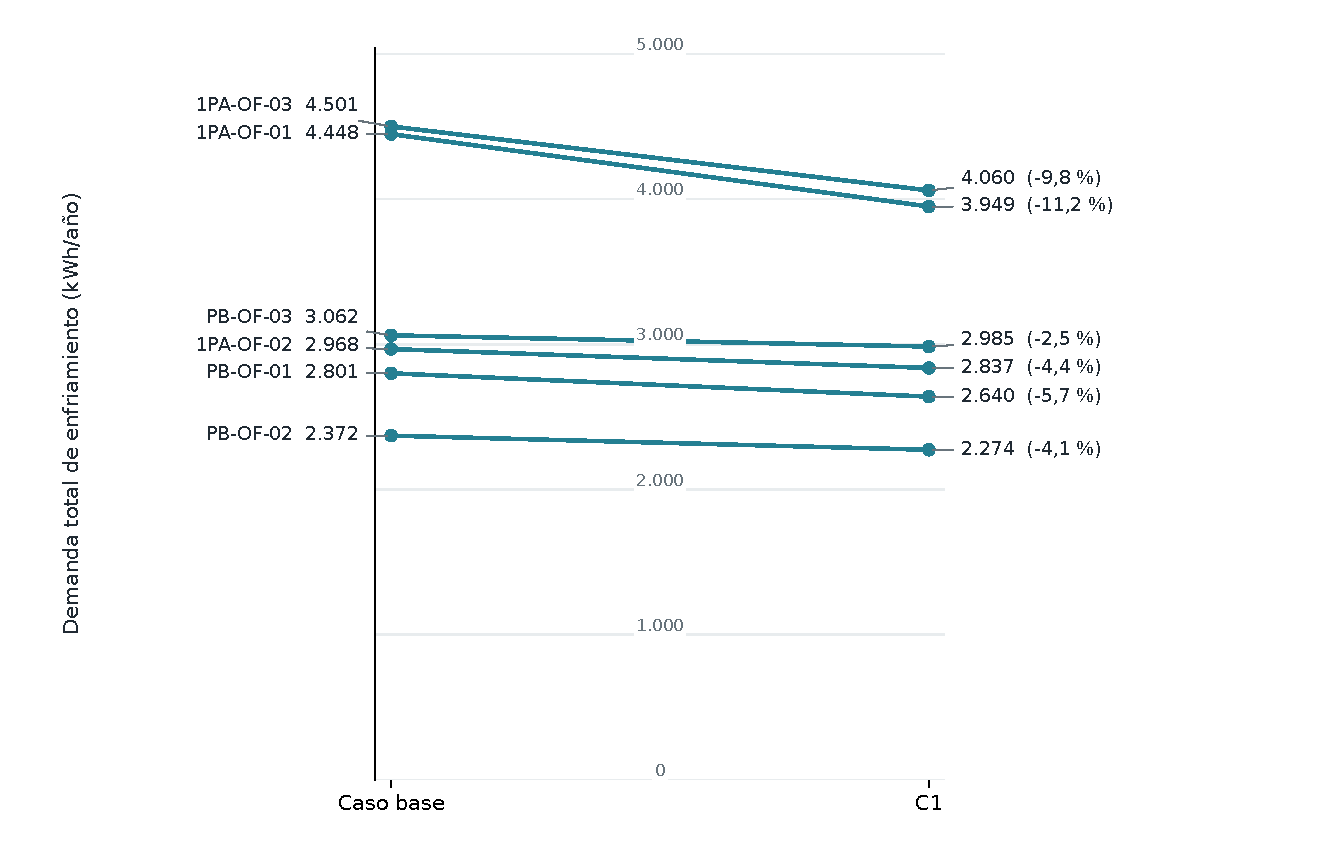
\includegraphics[width=\textwidth]{figuras/c1/03-cambio-oficinas.pdf}
\caption{Comparación de la demanda anual total de enfriamiento en las seis oficinas intervenidas.}
\label{fig:c1-oficinas-resultados}
\fuente{Elaboración propia con resultados de EnergyPlus, CB revisión 09 y C1 revisión 01. Valores en kWh térmicos por año; porcentajes referidos al CB de cada oficina.}
\end{figure}

La simulación conjunta no permite atribuir una fracción del ahorro a cada estrategia por separado. Para ello se requieren ensayos independientes de protección solar, apertura y control. Además, la disminución de demanda debe contrastarse con temperaturas durante la ocupación para descartar que responda a una reducción del servicio de refrigeración acompañada de menor confort.

\clearpage
\subsubsection{Distribución de aumentos y reducciones}
La figura~\ref{fig:c1-puntos-resultados} contabiliza las zonas con aumento, reducción o cambio no apreciable de demanda en cada mes. Cada punto tiene el mismo peso y representa una zona; por tanto, el número de puntos no expresa el volumen de energía ahorrada.
\begin{figure}[H]
\centering
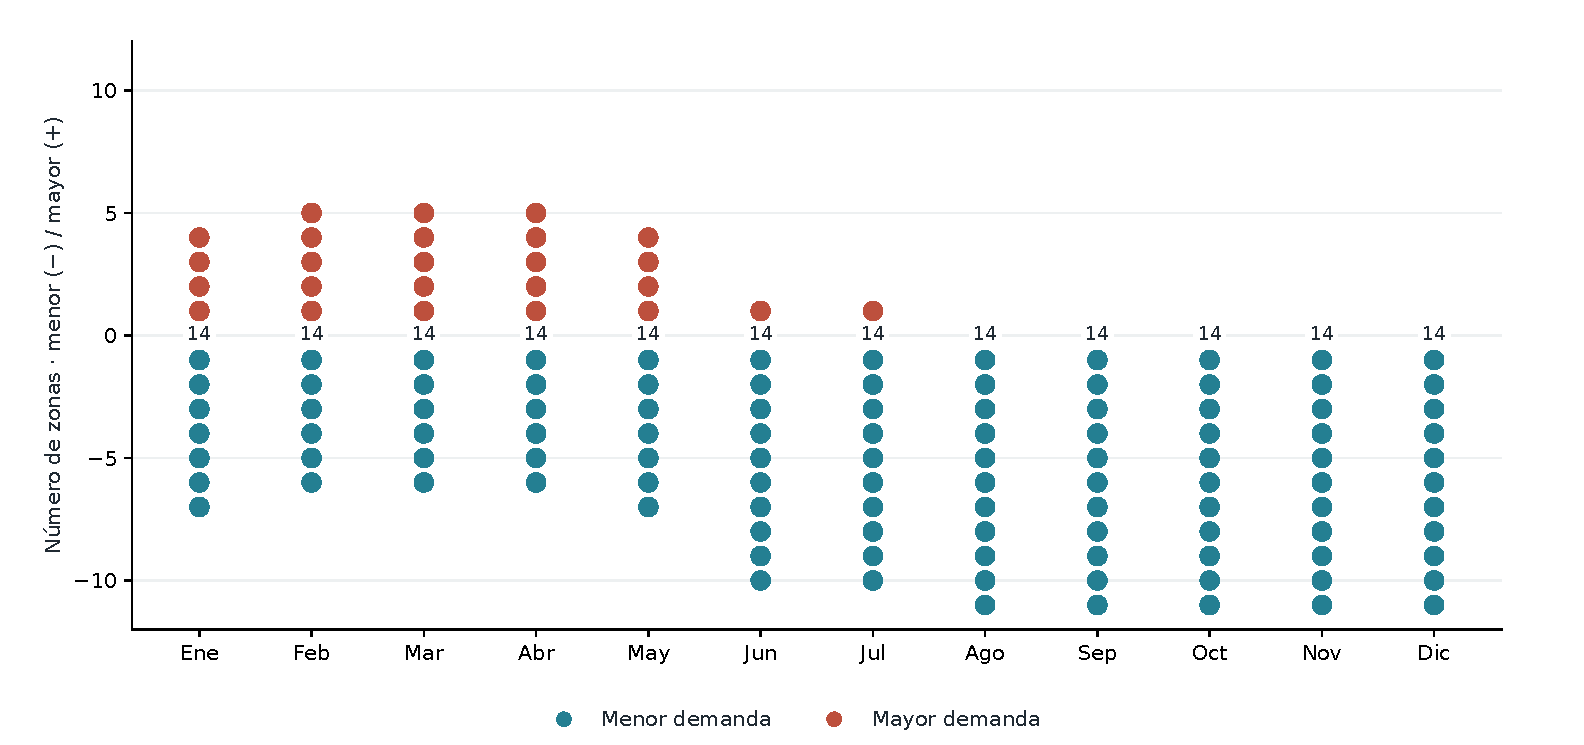
\includegraphics[width=\textwidth]{figuras/c1/04-zonas-por-mes.pdf}
\caption{Número de zonas con mayor y menor demanda mensual de enfriamiento en C1.}
\label{fig:c1-puntos-resultados}
\fuente{Elaboración propia con resultados de EnergyPlus. Base constante: 25 zonas con resultado de enfriamiento. La cifra sobre el eje cero identifica cambios de magnitud menor o igual a 0,1 kWh por mes; es una tolerancia de lectura, no un umbral normativo.}
\end{figure}

La integración de las potencias medias horarias se contrastó con los valores del periodo anual del archivo de resultados. Las tablas conservan la precisión original en los archivos CSV; los valores publicados se redondean para facilitar su lectura. C2 y C3 se presentan a continuación con resultados de sus propias corridas anuales.
\clearpage

\clearpage
\subsection{Ensayos independientes C2 y C3 y comparación conjunta}
\label{sec:escenarios-conjuntos}
C2 evalúa un acabado hipotético de cubierta con absortancia solar de 0,40 a 0,20 sobre 136,48 m\textsuperscript{2} brutos. C3 incorpora ese mismo cambio al paquete completo de C1: tres aleros de 0,50 m, fracción practicable del 20\,\% y control de ventilación natural y modo mixto en seis oficinas. Cada caso dispone de archivo y corrida anual propios. La orientación y la inercia térmica no fueron modificadas.

\begin{table}[H]\centering
\caption{Demanda total de enfriamiento y variación respecto al caso base}
{\small\singlespacing\renewcommand{\arraystretch}{1.3}
\begin{tabular}{lrrr}\toprule
Caso & kWh térmicos/año & Diferencia (kWh) & Variación (\%) \\ \midrule
CB & 84.759,41 & 0,00 & 0,00 \\
C1 & 83.103,76 & -1.655,65 & -1,95 \\
C2 & 84.328,85 & -430,56 & -0,51 \\
C3 & 82.748,96 & -2.010,45 & -2,37 \\
\bottomrule\end{tabular}}
\fuente{Elaboración propia con resultados de EnergyPlus: CB corrida 09 y C1, C2 y C3 revisión 01. Año 2025, mismo archivo climático. Resultados preliminares.}
\end{table}
C3 presenta una variación de -2,37\,\% frente al CB. La diferencia entre C3 y C1 es de -354,80 kWh térmicos al año. La interacción entre paquetes, definida como el ahorro combinado menos la suma de los ahorros independientes, es -75,76 kWh térmicos al año; no se asume aditividad.
La comparación integra potencias medias horarias durante 8.760 horas y concuerda con los registros del periodo anual. La demanda térmica no equivale a electricidad medida. Los valores no acreditan por sí solos una mejora del confort ni de la sostenibilidad de los materiales.
\clearpage
\begin{figure}[H]\centering
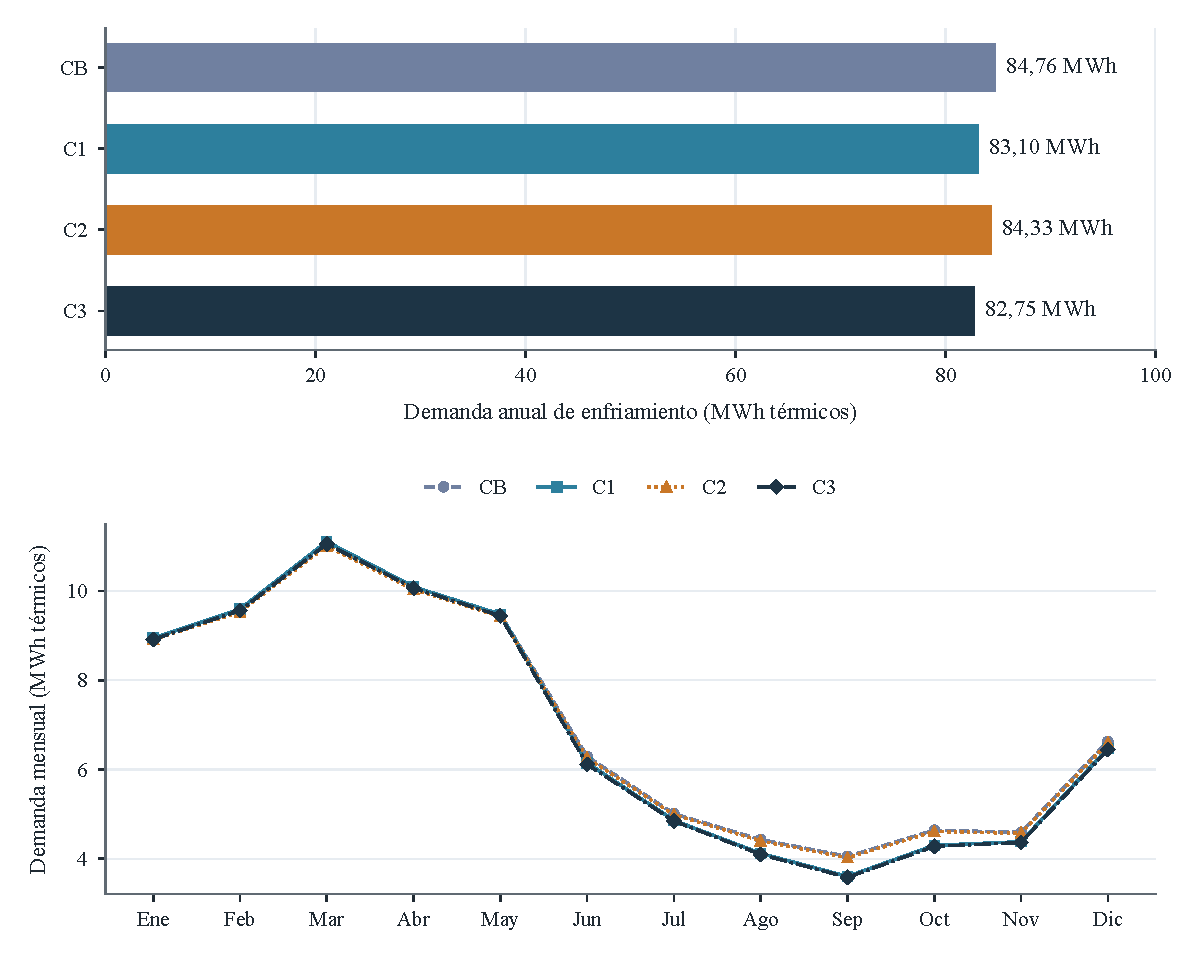
\includegraphics[width=\textwidth]{figuras/escenarios/comparacion-anual-mensual.pdf}
\caption{Demanda anual y mensual de enfriamiento de los cuatro escenarios.}
\fuente{Elaboración propia con las cuatro simulaciones independientes. Los colores identifican casos, no niveles de cumplimiento; los trazos y marcadores permiten distinguirlos también en escala de grises.}
\end{figure}
\begin{figure}[H]\centering
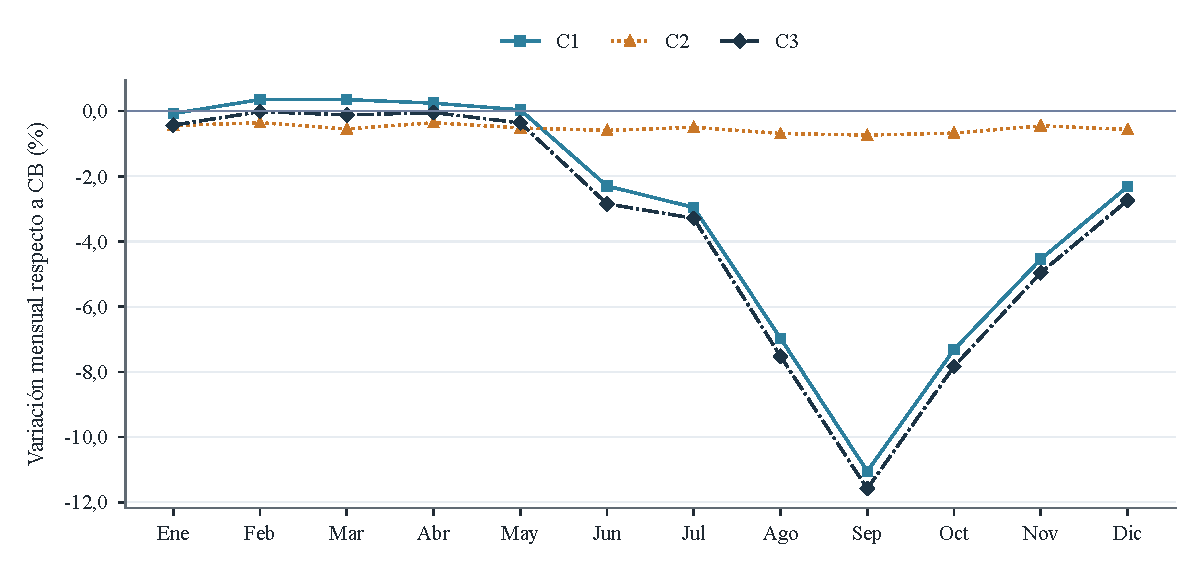
\includegraphics[width=\textwidth]{figuras/escenarios/variacion-mensual.pdf}
\caption{Variación mensual de enfriamiento de cada ensayo respecto al caso base.}
\fuente{Elaboración propia. Variación = 100 $\times$ (caso $-$ CB) / CB de cada mes. Los porcentajes mensuales no se promedian para obtener el ahorro anual.}
\end{figure}
\clearpage
\subsection{Correspondencia con la metodología y límites del alcance ejecutado}
\label{sec:control-metodologico}
La revisión del capítulo 3 distingue la ejecución energética de la verificación integral de sostenibilidad. El esquema de cuatro archivos independientes se mantiene, pero el alcance material todavía es parcial: C2 y C3 ensayan reflectancia y no acreditan contenido reciclado, bajo carbono ni menor huella ambiental. Esta diferencia respecto al alcance previsto se conserva expresamente y no se sustituye por una conclusión ambiental basada solo en energía.

\begin{table}[H]\centering
\caption{Verificación del alcance metodológico en los escenarios ejecutados}
{\small\singlespacing\renewcommand{\arraystretch}{1.2}
\begin{tabular}{p{3.2cm}p{2.1cm}p{8.1cm}}\toprule
Componente & Estado & Evidencia o trabajo pendiente \\ \midrule
Comparabilidad & Verificado & Mismo EPW y calendario anual; C3 conserva las medidas C1 y el acabado C2. Se documentan diferencias menores de importación frente al CB. \\
Demanda térmica & Ejecutado & Cuatro corridas propias y conciliación de resultados horarios y anuales. \\
Materiales sostenibles & No acreditado & Ficha comercial, reflectancia envejecida, cantidades, durabilidad y datos ambientales comparables pendientes. \\
Confort ocupado & Pendiente & Definir criterio de evaluación, horario por zona y horas de cumplimiento para los cuatro casos. \\
Iluminación & Parcial & Recalcular C1 y C3 con idéntica malla, cielo y plano de trabajo; los aleros pueden modificar la luz natural. \\
Validez física & Parcial & Revisar supuestos del datacenter, dimensionamiento y advertencias comunes del modelo. Cero errores severos no equivale a validación física. \\
Viabilidad & Pendiente & Disponibilidad, compatibilidad, mantenimiento, transporte y costes del acabado. \\
\bottomrule\end{tabular}}
\fuente{Elaboración propia: contraste entre el capítulo 3 y los modelos y resultados trazables de CB, C1, C2 y C3.}
\end{table}
La importación conserva áreas agregadas, pero modifica el área explícita de suelo del atrio superior de 6,2248 a 6,2174 m\textsuperscript{2} y el volumen del pasillo de segunda planta alta de 27,848 a 27,8479 m\textsuperscript{3}. Estas diferencias se registran como limitación de comparabilidad. Si se corrigen entradas comunes del CB, se deberán repetir los cuatro casos antes de considerar definitivos los porcentajes.
\clearpage

\clearpage
\subsection{Verificación de C3 revisión 02}
\label{sec:c3r02-resultados}
La revisión ampliada reduce la demanda total de enfriamiento de 84.759,41 a 65.767,88 kWh térmicos/año: una diferencia de 18.991,53 kWh y una reducción del 22,41\,\% respecto al caso base. Frente a C3 revisión 01, disminuye 16.981,08 kWh térmicos/año adicionales. El resultado corresponde al paquete conjunto de envolvente e iluminación; no permite atribuir el ahorro a un componente aislado.
\begin{table}[H]\centering
\caption{Resultado anual de la propuesta ampliada}
{\small\singlespacing\renewcommand{\arraystretch}{1.3}
\begin{tabular}{lrr}\toprule
Caso & Enfriamiento (kWh térmicos/año) & Reducción frente al CB (\%) \\ \midrule
Caso base & 84.759,41 & 0,00 \\
C3 revisión 01 & 82.748,96 & 2,37 \\
C3 revisión 02 & 65.767,88 & 22,41 \\
\bottomrule\end{tabular}}
\fuente{Elaboración propia con series horarias de EnergyPlus, calendario 2025 y clima común. Demanda térmica, no consumo eléctrico medido.}
\end{table}
La corrida finalizó con cero errores severos y 324 advertencias. Se amplió el máximo de días de inicialización de 25 a 100 para resolver la falta de convergencia inicial, conservando las tolerancias térmicas. La integración de 8.760 valores horarios coincide con el reporte anual, con diferencia inferior a 0,01 kWh. El cotejo con C3 revisión 01 confirma la conservación de geometría, clima, ocupación, equipos, horarios y consignas.

De los 19 controles de luz natural configurados, seis son ignorados por el motor porque sus zonas no tienen ventanas exteriores: PB-BO-01, PB-BA-01, PB-RE-01, 1PA-DC, 2PA-CAF y 2PA-PAS. La potencia de 8 W/m\textsuperscript{2} sí se aplica a las 19 zonas. El proyecto debe definir controles de presencia u otra solución apropiada para esos seis espacios y comprobar la cobertura exigida por E05. Las advertencias comunes de dimensionamiento y los supuestos del datacenter siguen siendo límites de la evaluación.

El 22,41\,\% cuantifica E01 frente al CB del proyecto. No acredita el umbral EDGE de E02, cuya referencia y balance de energía operacional requieren un cálculo específico. Tampoco demuestra por sí solo cumplimiento de confort ni certificación ambiental de los materiales.
\clearpage
\begin{figure}[H]\centering
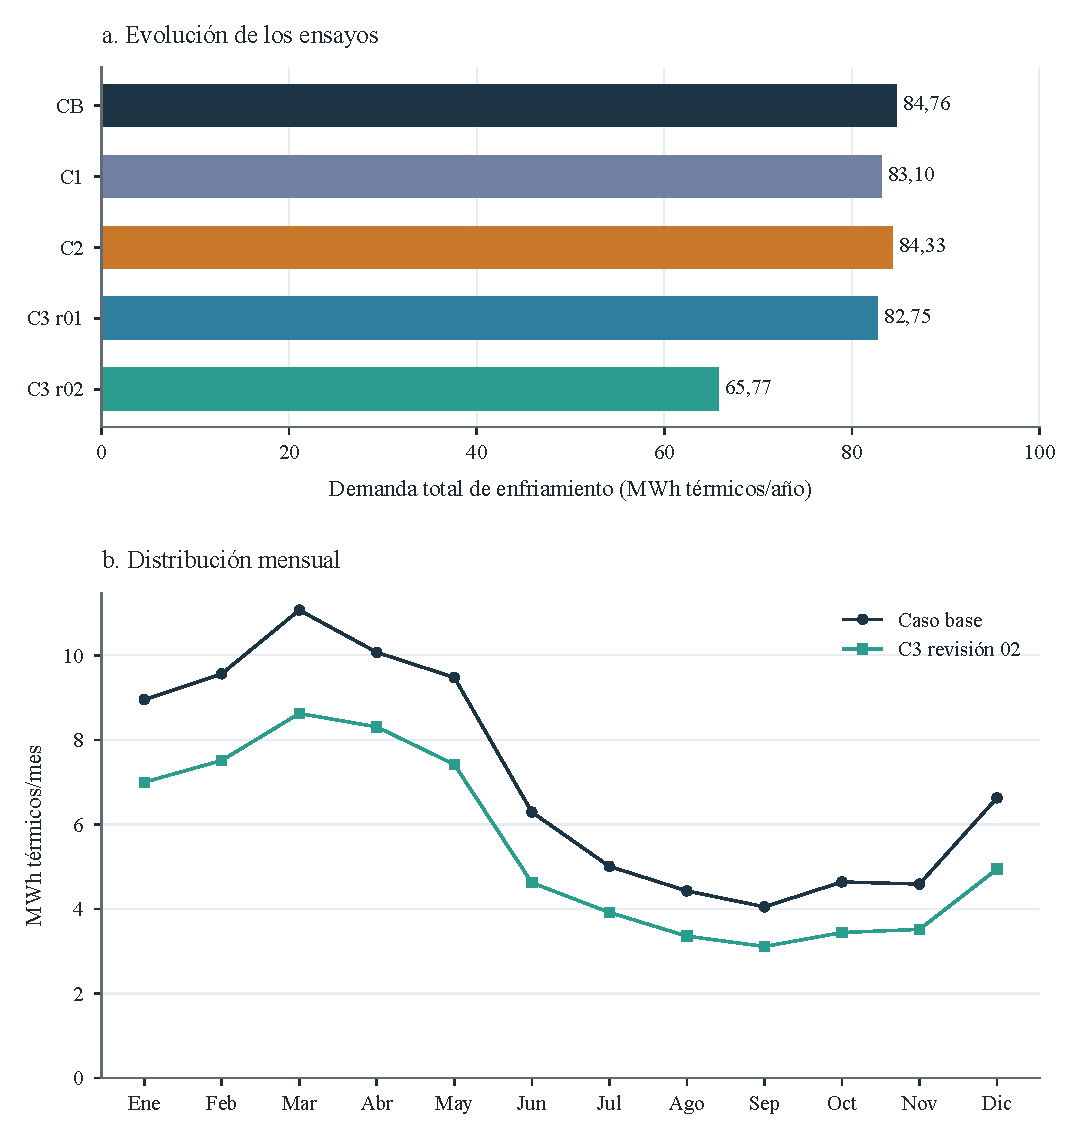
\includegraphics[width=0.94\textwidth]{figuras/escenarios/C3r02-comparacion.pdf}
\caption{Comparación anual de los ensayos y demanda mensual de la propuesta ampliada.}
\fuente{Elaboración propia con resultados de las cinco corridas. C3 r01 y C3 r02 son revisiones independientes; los colores identifican escenarios.}
\end{figure}
\clearpage
\begin{figure}[H]\centering
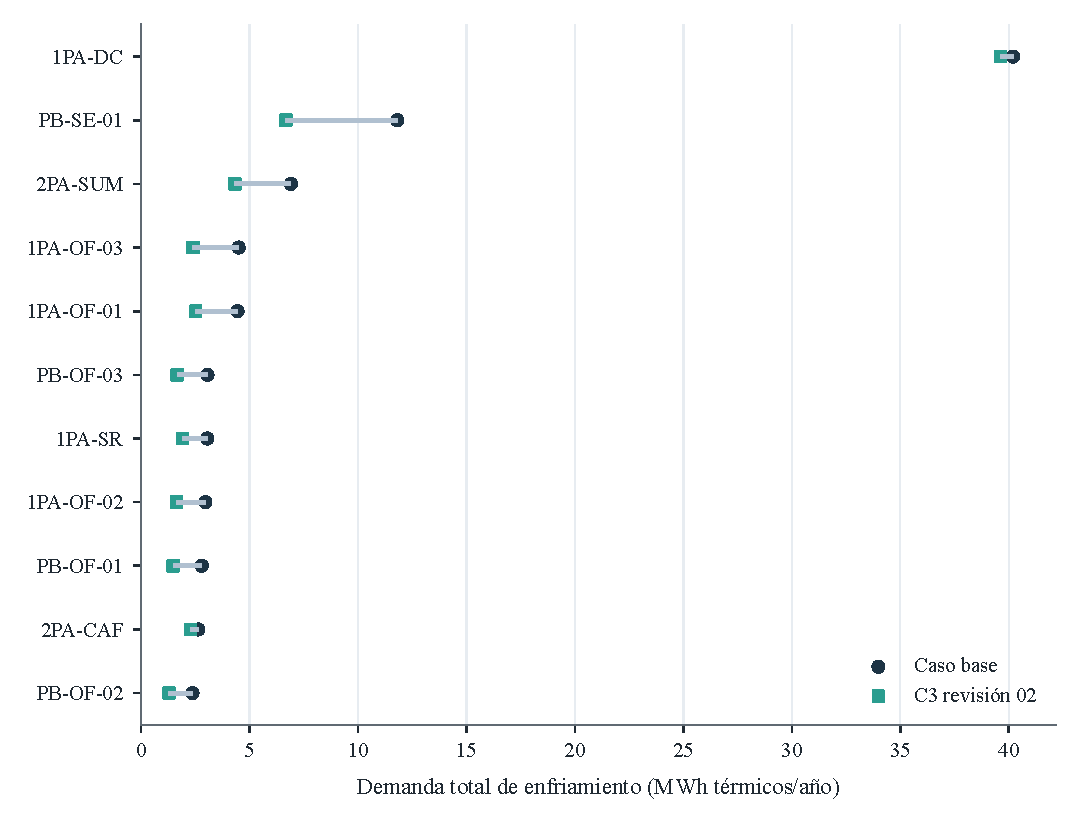
\includegraphics[width=\textwidth]{figuras/escenarios/C3r02-zonas.pdf}
\caption{Demanda anual de enfriamiento por zona: caso base y C3 revisión 02.}
\fuente{Elaboración propia. Se muestran las once zonas con demanda de enfriamiento distinta de cero en al menos uno de los dos modelos.}
\end{figure}
La comparación por zona permite localizar la respuesta del paquete y revisar los espacios con cargas internas persistentes. La permanencia de una demanda elevada no debe resolverse modificando arbitrariamente las cargas para obtener un porcentaje de ahorro mayor; requiere contrastar el uso y el equipamiento con el programa real del edificio.

\par\medskip
\subsection{Respuesta térmica durante la ocupación de oficinas}
La temperatura operativa se compara en las seis oficinas intervenidas mediante 3.130 intervalos horarios ocupados por zona: lunes a sábado, de 08:00 a 18:00, según el calendario 2025 del modelo, sin festivos adicionales. Se conservan los mismos horarios en ambas corridas. El percentil 95 describe la parte alta de la distribución; no es un umbral normativo de confort.
\begin{table}[H]\centering
\caption{Temperatura operativa en horas ocupadas: caso base y C3 revisión 02}
{\small\singlespacing\renewcommand{\arraystretch}{1.25}
\begin{tabular}{lrrrrr}\toprule
 & \multicolumn{2}{c}{Media (\textdegree C)} & \multicolumn{2}{c}{P95 (\textdegree C)} & \\
Oficina & CB & C3 r02 & CB & C3 r02 & $\Delta$ media (K) \\ \midrule
PB-OF-01 & 26,75 & 26,02 & 28,36 & 27,04 & -0,74 \\
PB-OF-02 & 26,98 & 26,14 & 28,56 & 27,24 & -0,85 \\
PB-OF-03 & 26,83 & 26,08 & 28,34 & 27,10 & -0,75 \\
1PA-OF-01 & 27,17 & 26,28 & 28,91 & 27,68 & -0,89 \\
1PA-OF-02 & 27,07 & 26,26 & 28,15 & 27,24 & -0,80 \\
1PA-OF-03 & 26,83 & 25,97 & 28,23 & 27,21 & -0,85 \\
\bottomrule\end{tabular}}
\fuente{Elaboración propia con series horarias de EnergyPlus y horarios de ocupación del modelo. $\Delta$ = C3 r02 $-$ CB.}
\end{table}
Estos estadísticos cuantifican la respuesta térmica, pero no acreditan C01. La evaluación de confort requiere separar las horas de funcionamiento mecánico y natural, aplicar el método correspondiente y comprobar sus condiciones de actividad, vestimenta, velocidad del aire y cobertura espacial. Una reducción de demanda o de temperatura media no equivale automáticamente a mayor porcentaje de horas confortables.


\clearpage
\section{Respuesta a la matriz y alcance de los objetivos}
\subsection{Respuesta de los escenarios a la matriz y estado de los objetivos}
\label{sec:matriz-escenarios}
Las corridas de la revisión 01 cuantifican E01: C1 reduce la demanda total de enfriamiento un 1,95\,\%, C2 un 0,51\,\% y C3 un 2,37\,\% respecto al CB. Este indicador comparativo no se transforma en cumplimiento de E02, que requiere energía operacional y referencia EDGE. Tampoco permite resolver C01 sin evaluar condiciones térmicas ocupadas.

C1 y C3 incorporan medidas relacionadas con E04 y P01, pero falta verificar su protección solar eficaz, área neta de abertura e incidencia lumínica anual. C2 y C3 modifican la absortancia de cubierta de 0,40 a 0,20; M01 permanece no evaluable porque no hay cantidades y factores ambientales del producto que acrediten menor carbono incorporado. Un cambio óptico no sustituye una selección de materiales sostenibles.

C3 revisión 02 responde a las brechas de envolvente e iluminación mediante nuevos parámetros y una corrida independiente (sección~\ref{sec:c3-revision02}). Su reducción térmica frente al CB es del 22,41\,\%. El cumplimiento completo de E03 y E05 exige, además, detalles constructivos, fotometría y solución de control para las seis zonas sin ventanas exteriores. Los indicadores de agua, materiales, equipos y operación se vinculan con el plan de cierre; una especificación propuesta no cambia automáticamente su estado a cumplimiento.

\begin{table}[H]\centering
\caption{Estado de desarrollo de los objetivos específicos}
{\small\singlespacing\renewcommand{\arraystretch}{1.3}\setlength{\tabcolsep}{4pt}
\begin{tabular}{>{\raggedright\arraybackslash}p{1.6cm}>{\raggedright\arraybackslash}p{3.2cm}>{\raggedright\arraybackslash}p{9.1cm}}\toprule
Objetivo & Estado documental & Evidencia y condición pendiente \\ \midrule
OE1 & Matriz configurada & 16 indicadores, cinco marcos, reglas y fuentes explícitas. Pendiente contraste externo de pertinencia y confirmación de condiciones de aplicación. \\
OE2 & Evaluación parcial & Matriz aplicada al CB, una brecha de iluminación identificada y límites registrados. Faltan datos para completar confort, aire, agua, materiales y otros criterios. \\
OE3 & Propuesta preliminar & Paquete pasivo y acabado reflectante simulados; revisión 02 amplía envolvente e iluminación. Falta selección ambiental demostrada y cierre de los criterios restantes. \\
OE4 & Validación parcial & Demanda térmica comparada en cinco corridas y temperatura operativa ocupada de seis oficinas contrastada entre CB y C3 r02. Se cuantificaron horas con PMV $\pm0,5$; resta separar regímenes de operación y ampliar la cobertura espacial. \\
\bottomrule\end{tabular}}
\fuente{Elaboración propia a partir de las simulaciones y de la matriz de indicadores. Los estados no son calificaciones de certificación.}
\end{table}


\section{Implementación y lineamientos replicables}
El plan relaciona los 16 indicadores del capítulo 3 con tareas de diseño y evidencia de cierre. Los responsables son roles propuestos, no contrataciones confirmadas. La definición de una especificación no equivale a su cumplimiento construido.
\clearpage
\subsection{Energía y calidad ambiental}
\begin{table}[H]\centering
\caption{Acciones de implementación y evidencia requerida: energía y calidad ambiental}
{\fontsize{9}{11}\selectfont\singlespacing\renewcommand{\arraystretch}{1.3}
\begin{tabular}{>{\raggedright\arraybackslash}p{1.1cm}>{\raggedright\arraybackslash}p{6.1cm}>{\raggedright\arraybackslash}p{6.1cm}}\toprule
ID & Acción y responsable propuesto & Evidencia de cierre \\ \midrule
E01 & Comparar CB y C3r02 con entradas comunes y nuevas cargas de diseño. Simulación. & Series horarias conciliadas y reducción anual. \\
E02 & Construir referencia EDGE y contabilizar todos los usos y sistemas reales. Especialista energético. & Ahorro operacional mínimo del 20 \,\% frente a referencia EDGE. \\
E03 & Resolver aislamiento continuo, puentes térmicos y humedad. Confirmar clima y compacidad. Arquitectura. & Memoria de U del conjunto y detalles constructivos. \\
E04 & Comprobar cada orientación y ajustar aleros o lamas sin anular luz natural. Arquitectura. & SHGC modificado $<$0,20 en al menos 90 \,\% de superficies aplicables. \\
E05 & Especificar LED y verificar regulación, lux y cobertura del control. Diseño eléctrico. & Potencia $\leq$8 W/m\textsuperscript{2}; fotometría y control según matriz. \\
C01 & Evaluar horas ocupadas por zona y separar funcionamiento mecánico y natural. Simulación. & PMV o método adaptativo aplicable; porcentaje espacial y temporal. \\
C02 & Dimensionar aire exterior, filtración y recuperación; verificar condiciones de excepción. Diseño HVAC. & Memoria de caudales y equipos según T4 y normativa aplicable. \\
C03 & Calcular sDA y ASE con la misma malla, ocupación y plano de trabajo. Simulación lumínica. & Resultados anuales y tratamiento del deslumbramiento. \\
\bottomrule\end{tabular}}
\fuente{Elaboración propia con los umbrales y condiciones de la matriz del capítulo 3.}
\end{table}
\clearpage
\subsection{Recursos, sistemas y operación}
\begin{table}[H]\centering
\caption{Acciones de implementación y evidencia requerida: recursos, sistemas y operación}
{\fontsize{9}{11}\selectfont\singlespacing\renewcommand{\arraystretch}{1.3}
\begin{tabular}{>{\raggedright\arraybackslash}p{1.1cm}>{\raggedright\arraybackslash}p{6.1cm}>{\raggedright\arraybackslash}p{6.1cm}}\toprule
ID & Acción y responsable propuesto & Evidencia de cierre \\ \midrule
A01 & Seleccionar griferías y sanitarios eficientes con caudales a presión de ensayo. Diseño sanitario. & Balance de usuarios y ahorro $\geq$20 \,\% respecto a referencia EDGE. \\
M01 & Medir cantidades y comparar EPD con igual unidad funcional y límites. Arquitectura y presupuesto. & Balance EDGE de materiales; reducción $\geq$20 \,\% demostrada. \\
M02 & Solicitar ensayos de emisiones para acabados, adhesivos y aislantes. Especificación y compras. & Expediente de todos los productos de la intervención. \\
E06 & Determinar SRE, área útil sin sombras y demanda eléctrica. Diseño eléctrico. & Potencia mínima según T2; diseño eléctrico y estructural. \\
E07 & Seleccionar equipos con SEER verificable y revisar dimensionamiento. Diseño HVAC. & SEER $\geq$6 y sobredimensionamiento $\leq$15 \,\%, según aplicación. \\
G01 & Asignar medición de energía, agua e indicadores interiores. Operación. & Plan con responsable, frecuencia y acciones correctivas. \\
G02 & Comparar suministro, transporte, salinidad, mantenimiento y reposición. Presupuesto y operación. & Cotizaciones y evaluación de ciclo de vida y logística. \\
P01 & Comprobar área libre respecto al suelo, seguridad y protección frente a lluvia. Arquitectura. & Abertura efectiva $\geq$4 \,\% en oficinas cuando aplique A6. \\
\bottomrule\end{tabular}}
\fuente{Elaboración propia con los umbrales y condiciones de la matriz del capítulo 3.}
\end{table}
\clearpage
\subsection{Lineamientos transferibles al contexto insular}
La secuencia replicable consiste en reducir primero las cargas evitables, comprobar después la respuesta de cada espacio y seleccionar finalmente sistemas y materiales con evidencia de suministro y mantenimiento. La potencia de iluminación debe vincularse con la tarea visual; la protección solar, con la orientación y la luz natural; y la ventilación, con el clima y los caudales efectivos.

Las transmitancias o fracciones de apertura de este ensayo no se trasladan automáticamente a otros edificios. Cada aplicación requiere geometría, clima, ocupación y condiciones constructivas propias. En Galápagos, la reposición, el transporte y la exposición ambiental forman parte de la selección técnica y de su viabilidad económica.


\section{Síntesis de la propuesta}
\begin{textoDosTercios}
La propuesta articula protección solar, ventilación controlada, envolvente con menor transmitancia e iluminación de menor potencia. La revisión 02 traduce brechas concretas de la matriz en parámetros verificables y mantiene un expediente independiente de los ensayos previos.

La selección constructiva exige compatibilidad con el edificio y con la logística de San Cristóbal. El aislamiento requiere continuidad, control de humedad y solución de fijaciones; el vidrio exige comprobar el conjunto con sus marcos; las luminarias necesitan una distribución fotométrica que satisfaga las tareas. La sostenibilidad de los materiales depende de cantidades, durabilidad y documentación ambiental comparable.

El alcance de la validación se limita a los indicadores respaldados por resultados y documentos trazables. La matriz orienta el proyecto, pero no constituye una certificación Minergie, WELL, EDGE o LEED. Los criterios pendientes se mantienen explícitos como condiciones de cierre del proyecto y de la investigación.
\end{textoDosTercios}
